\title[Causality]{Causality: Lecture 12}
\author[Joris Mooij]{\\[5mm]\large Joris Mooij \& Patrick Forr\'e\\
\url{j.m.mooij@uva.nl}, \url{p.d.forre@uva.nl}}
\institute[UvA]{University of Amsterdam}
\date[2025-04-24]{\normalsize April 24th, 2025}
\maketitle



\part{Counterfactuals}
\frame{\partpage}

\begin{frame}{Informal definition}
  A counterfactual statement invites one to imagine an alternative (counterfactual) world, in which 
  everything is the same as in the actual world, except that one aspect of it is changed.

  \begin{definition}[Informal]
We consider counterfactuals that are hypothetical statements regarding the effects of some action that is contrary-to-fact.
  \end{definition}

  We use our causal model of the world to predict the consequences of this imaginary change.

  \begin{example}
  Suppose you are healthy but drank too much beer last night and now suffer from a hangover. 
  A counterfactual statement is then: ``If I had not drunk so much beer yesterday, I would feel much better now.''
  \end{example}

  Counterfactual thinking is very common in humans, and toddlers already bombard
  their parents with counterfactual questions, presumably as a means for them
  to build internal causal models of the world.
\end{frame}

\begin{frame}{Twin iSCM}
  \begin{Def}[\ref{def:twin_scm}]
  Let $M = \lt \Sin, \Send, \Srnd, \CX, P, f \rt$ be an iSCM. We define its \emph{twinned iSCM} as
    $M^\twin = \lt \Sin^\twin = \Sin \dot\cup \Sin', \Send^\twin = \Send \dot\cup \Send', \Srnd, \CX^\twin, P, f^\twin \rt$
  with
  \begin{enumerate}
    \item $\Sin' = \{j' : j \in \Sin\}$ a copy of $\Sin$,
    \item $\Send' = \{v' : v \in \Send\}$ a copy of $\Send$,
    \item the twinned domain given by
  $$\CX^\twin = \CXJ \times \CX_{J'} \times \CXV \times \CX_{V'} \times \CXW$$
  where $\CX_{j'} = \CX_j$ for all $j \in J$ and $\CX_{v'} = \CX_v$ for all $v \in V$,
    \item the twinned causal mechanism components given by
      \vspace{-0.5\baselineskip}
    $$f^\twin_u\big((x_J,x_{J'}),(x_V,x_{V'}),\xW\big) = 
    \begin{cases}
      f_u(\xJ,\xV,\xW) & u \in \Send,  \\
      f_{u^\circ}(x_{J'},x_{V'},\xW) & u \in \Send'.
    \end{cases}$$
  \end{enumerate}
  \end{Def}
  This creates copies of some variables so that their values can differ in the counterfactual world with respect to the actual world.
\end{frame}


\begin{frame}{Counterfactuals: Example}
  \begin{example}
  Variables:\\
    \quad $T$ : number of hours studied (exogenous input variable)\\
%    \quad $E$ : study efficiency (exogenous input variable)\\
    \quad $D$ : exam difficulty (exogenous random variable)\\
    \quad $G$ : grade (endogenous variable)\\
  Structural equation:\\
  \smallskip
  \centerline{$G = f(T,D).$}
  \smallskip
  Counterfactual query: {\it ``I studied 20 hours for the exam and
got a 4.5; if I had studied 30 hours instead, what would have been my grade?''}\\

    \medskip
    Twin iSCM has copies $T'$ and $G'$, and structural equations:\\
    \smallskip
    \centerline{$G = f(T,D) \qquad G' = f(T',D).$}
    \smallskip
    The answer to the counterfactual query is:\\
    \smallskip
    \centerline{$P(G' \given \doit(T'=30), \doit(T=20), G=4.5)$}
    \smallskip
  \end{example}
\end{frame}

\begin{frame}{Discussion}
The English language has a grammatical construct for counterfactuals:\\
\quad ``If I had studied well, I would have passed the exam,''\\
instead of\\
\quad ``If I study well, I will pass the exam.''\\
For the former statement, we first twin the iSCM and then intervene on it, for the latter, we only intervene on the iSCM (no need for twinning!). 

\bigskip
So not only from the grammatical, but also from the modeling point of view, these are quite different questions!

\bigskip
\setbeamercolor{block title}{use=structure,fg=white,bg=purple!75!black}
\setbeamercolor{block body}{use=structure,fg=black,bg=white!20!white}
  \begin{block}{Warnings}
    \begin{itemize}
      \item
  Unfortunately, in large part of the causality literature, the term ``counterfactuals'' is also used 
  as a synonym for potential outcomes, which are not necessarily contrary-to-fact. This may
  cause confusion.
%  (for example, ``If you drink too much beer you will get a hangover'').
\item Generally, in situations where the full causal mechanism is unknown, or exogenous
randomness is latent, counterfactuals may be VERY model-dependent.
    \end{itemize}
  \end{block}
\end{frame}


\begin{frame}{Properties of the twinning operation I}
The twinning operation has the following properties.

%Let $M = \lt \Sin, \Send, \Srnd, \CX, P, f \rt$ and $\tilde{M} = \ltuple \Sin, \Send, \Srnd, \CX, P, \tilde{f} \rtuple$ be iSCMs.
%  \begin{Prp}[\ref{prp:twinning_preserves_scm_equivalence}]
%  Twinning preserves equivalence: $M \equiv \tilde{M} \implies M^\twin \equiv \tilde{M}^\twin$.
%  \end{Prp}
Let $M = \lt \Sin, \Send, \Srnd, \CX, P, f \rt$ be an iSCM.
Twinning preserves equivalence: $M \equiv \tilde{M} \implies M^\twin \equiv \tilde{M}^\twin$.
  \begin{Prp}[\ref{prp:twinning_marginalization_commute}]
Let $M = \lt \Sin, \Send, \Srnd, \CX, P, f \rt$ be an iSCM.
  If $M$ is essentially uniquely solvable w.r.t.\ $L \ins V$,
  $$(M_{\setminus L})^\twin = (M^\twin)_{\setminus (L\cup L')}.$$
  \end{Prp}
  \begin{Cor}[\ref{prp:twin_scm_simple}]
  Let $M = \lt \Sin, \Send, \Srnd, \CX, P, f \rt$ be an iSCM.
    \begin{itemize}
      \item If $M$ is essentially uniquely solvable, then $M^\twin$ is essentially uniquely solvable.
      \item If $M$ is simple, then $M^\twin$ is simple.
    \end{itemize}
  \end{Cor}
\end{frame}

\begin{frame}{Properties of the twinning operation II}
Hard interventions are compatible with twinning:
\begin{Prp}[\ref{prp:hard_interventions_twin_scm}]
Let $M = \lt \Sin, \Send, \Srnd, \CX, P, f \rt$ be an iSCM.
\begin{itemize}
  \item For $T \subseteq \Sin \cup \Send$, $\xT \in \CXT$:
    $$(M^\twin)_{\doit(X_T=\xT,X_{T'}=\xT)} = (M_{\doit(\XT=\xT)})^\twin.$$
%  \item For $T \subseteq \Srnd$, $Q_T \in \prod_{t\in T} \C{P}(\CX_t)$:
%    $$(M^\twin)_{\doit(X_T\sim Q_T)} = (M_{\doit(\XT\sim Q_T)})^\twin.$$
  \item For $T \subseteq \Sin \cup \Send$:
    $$(M^\twin)_{\doit(T,T')} = (M_{\doit(T)})^\twin.$$
  \item For $T \ins J \cup V$:
    $$(M^\twin)_{\doit(I_T,I_{T'})} = (M_{\doit(I_T)})^\twin$$
    (where we identify $I_t'$ with $I_{t'}$ for all $t \in T$). 
\end{itemize}
\end{Prp}
\end{frame}

\begin{frame}{Graphical twinning operation}
We can also define a twinning operation on graphs.
\begin{Def}[\ref{def:G_twinning}]
  Let $G=\lt J,V \cup W,E\rt$ be a CDG such that $\Pa^G(W) = \emptyset$. Write $J' := \{j' : j \in J\}$
  and $V' := \{v' : v \in V\}$ for copies of $J$ and $V$.
  The \emph{twinned graph
  $G^{\twin(J,V)}$} is defined as the CDG $\lt J \dot\cup J', V \dot\cup V' \cup W, E^\twin\rt$ with directed edges
  \begin{equation*}\begin{split}
    E^\twin := E & \cup \{w \tuh v' : w \in W, v \in V, w \tuh v \in E\}\\
                 & \cup \{i' \tuh v' : i \in J \cup V, v \in V, i \tuh v \in E\}.
  \end{split}\end{equation*}
\end{Def}
In words, we copy the nodes $J \cup V$ (but not the nodes $W$) and copy the edges accordingly.
The graphical and the iSCM twinning operations are compatible:
\begin{Prp}[\ref{prp:compatibility_graph_twinning}]
  For iSCM $M = \lt \Sin, \Send, \Srnd, \CX, P, f \rt$, $(G^+(M))^{\twin(J\cup V)} = G^+(M^\twin).$
\end{Prp}
\end{frame}

\begin{frame}{Example of graphical twinning operation}
  \begin{Eg}
  Consider an iSCM $M$ with exogenous input variable $X$, endogenous variable $Y$, exogenous random variable $W$, and
  structural equation\\

  \smallskip
  \qquad $Y^{\doit(x)} = f(x,W)$.\\

  \smallskip
  Twinning adds an exogenous input variable $X'$, an endogenous variable $Y'$, and structural equation\\

  \smallskip
  \qquad $(Y')^{\doit(x')} = f(x',W)$,\\
  
  \smallskip
  but keeps the same endogenous random variable $W$.

    \centerline{\begin{tikzpicture}
    \begin{scope}
      \node[ndint] (X) at (0,0) {$X$};
      \node[ndout] (Y) at (0,-1.5) {$Y$};
      \node[ndlat] (W) at (1,-0.75) {$W$};
      \draw[arint] (X) to (Y);
      \draw[arout] (W) to (Y);
      \node at (0,-2.5) {$G^+(M)$};
    \end{scope}
    \begin{scope}[xshift=5cm]
      \node[ndint] (X) at (0,0) {$X$};
      \node[ndout] (Y) at (0,-1.5) {$Y$};
      \node[ndlat] (W) at (1,-0.75) {$W$};
      \draw[arint] (X) to (Y);
      \draw[arout] (W) to (Y);
      \node[ndint] (X2) at (2,0) {$X'$};
      \node[ndout] (Y2) at (2,-1.5) {$Y'$};
      \draw[arint] (X2) to (Y2);
      \draw[arout] (W) to (Y2);
      \draw[dotted] (-1,-2) rectangle (1,0.5);
      \draw[dotted] (1,-2) rectangle (3,0.5);
      \node at (0,0.8) {\tiny factual};
      \node at (2,0.8) {\tiny counterfactual};
      \node at (1,-2.5) {$G^+(M^{\twin}) = (G^+(M))^{\twin(X,Y)}$};
    \end{scope}
    \end{tikzpicture}}
  \end{Eg}
\end{frame}

\begin{frame}{Other types of counterfactuals?}
  Not all counterfactual statements are naturally modeled via twinning.
  E.g., if circumstances are hypothesized to be different, then this may not necessarily correspond to an intervention.
  \begin{Eg}
    ``Yesterday I met an old friend in the street that I hadn't seen in years. 
    We decided to go have a beer in the pub, even though I had plans to study for my exam that night. 
    If I had not bumped into my old friend, I would not have ended up in the pub yesterday evening.''
  \end{Eg}
  This is an example of a \emph{backtracking} counterfactual.
  We do not attempt to formalize backtracking counterfactuals here.
\end{frame}

\part{Counterfactual Equivalence}
\frame{\partpage}

\begin{frame}{Counterfactual equivalence: definition}
  \begin{Def}[\ref{def:scm_counterfactual_equiv}]
  Let $M = \lt \Sin, \Send, \Srnd, \CX, P, f \rt$ and
  $\tilde{M} = \ltuple \tilde{\Sin}, \tilde{\Send}, \tilde{\Srnd}, \tilde{\CX}, \tilde{P}, \tilde{f} \rtuple$ be two simple iSCMs
  and $O \subseteq \Send \cap \tilde{\Send}$ a subset.
  We say that:
  \begin{enumerate}
    \item {\color{gray}$M$ and $\tilde{M}$ are \emph{observably equivalent w.r.t.\ $O$} if $\CX_O = \tilde{\CX}_O$, $\CX_{J\cap\tilde{J}} = \C{\tilde{X}}_{J\cap\tilde{J}}$, and $P_{M}(X_O \mid \doit(\XJ)) = P_{\tilde{M}}(X_O \mid \doit(\CX_{\tilde{J}}))$;}
    \item {\color{gray}$M$ and $\tilde{M}$ are \emph{interventionally equivalent w.r.t.\ $O$} if for every subset $T \subseteq O$ the intervened iSCMs $M_{\doit(T)}$ and $\tilde{M}_{\doit(T)}$ are observably equivalent w.r.t.\ $O \setminus T$;}
    \item $M$ and $\tilde{M}$ are \emph{counterfactually equivalent w.r.t.\ $O$} if the twin iSCMs $M^\twin$ and $\tilde{M}^\twin$ are interventionally equivalent w.r.t.\ $O \cup O'$, where
    $O'$ is the copy of $O$ in $V' \cap \tilde{V}'$.
  \end{enumerate}
  \end{Def}
\end{frame}

\begin{frame}{Marginalization preserves counterfactual semantics}
  \begin{Cor}[\ref{Cor:various_equiv_marginalization}]
  If $M = \lt \Sin, \Send, \Srnd, \CX, P, f \rt$ is simple, $L \subseteq \Send$, and
  $M_{\setminus L}$ is its marginalization over $L$. Then $M$ and $M_{\setminus L}$ are {\color{gray}observably,
  interventionally and} counterfactually equivalent w.r.t.\ $V \setminus L$.
  \end{Cor}
\begin{proof}
  Write $K := V \setminus L$.
  Note that $(M_{\setminus L})^\twin = (M^\twin)_{\setminus (L \cup L')}$. 
  Since $M^\twin$ and its marginalization
  $(M^\twin)_{\setminus (L \cup L')}$ are interventionally equivalent w.r.t.\ $K \cup K'$,
  $M$ and $M_{\setminus L}$ are counterfactually equivalent w.r.t.\ $K$.
\end{proof}
\end{frame}

\begin{frame}{Implications between equivalences}
  \begin{Prp}[\ref{prp:equivalence_implies_counterf_equiv},\ref{prp:pearls_ladder_levels_2_and_3}]
  For simple iSCMs $M, \tilde{M}$ and a subset $O \subseteq \Send \cap \tilde{\Send}$:
  \begin{enumerate}
    \item If $M \equiv \tilde{M}$ then $M$ and $\tilde{M}$ are counterfactually equivalent w.r.t.\ $O$.
    \item If $M$ and $\tilde{M}$ are counterfactually equivalent w.r.t.\ $O$ then 
      $M$ and $\tilde{M}$ are interventionally equivalent w.r.t.\ $O$.
    \item {\color{gray}If $M$ and $\tilde{M}$ are interventionally equivalent w.r.t.\ $O$ then 
      $M$ and $\tilde{M}$ are observably equivalent w.r.t.\ $O$.}
  \end{enumerate}
\end{Prp}
The reverse implications do not hold in general. This expresses that causal modeling is more refined than
probabilistic modeling, and counterfactual modeling is more refined than interventional modeling.
\end{frame}

\begin{frame}{Pearl's Ladder of Causation}
  \centering
  \begin{tikzpicture}
    \node (0,0) {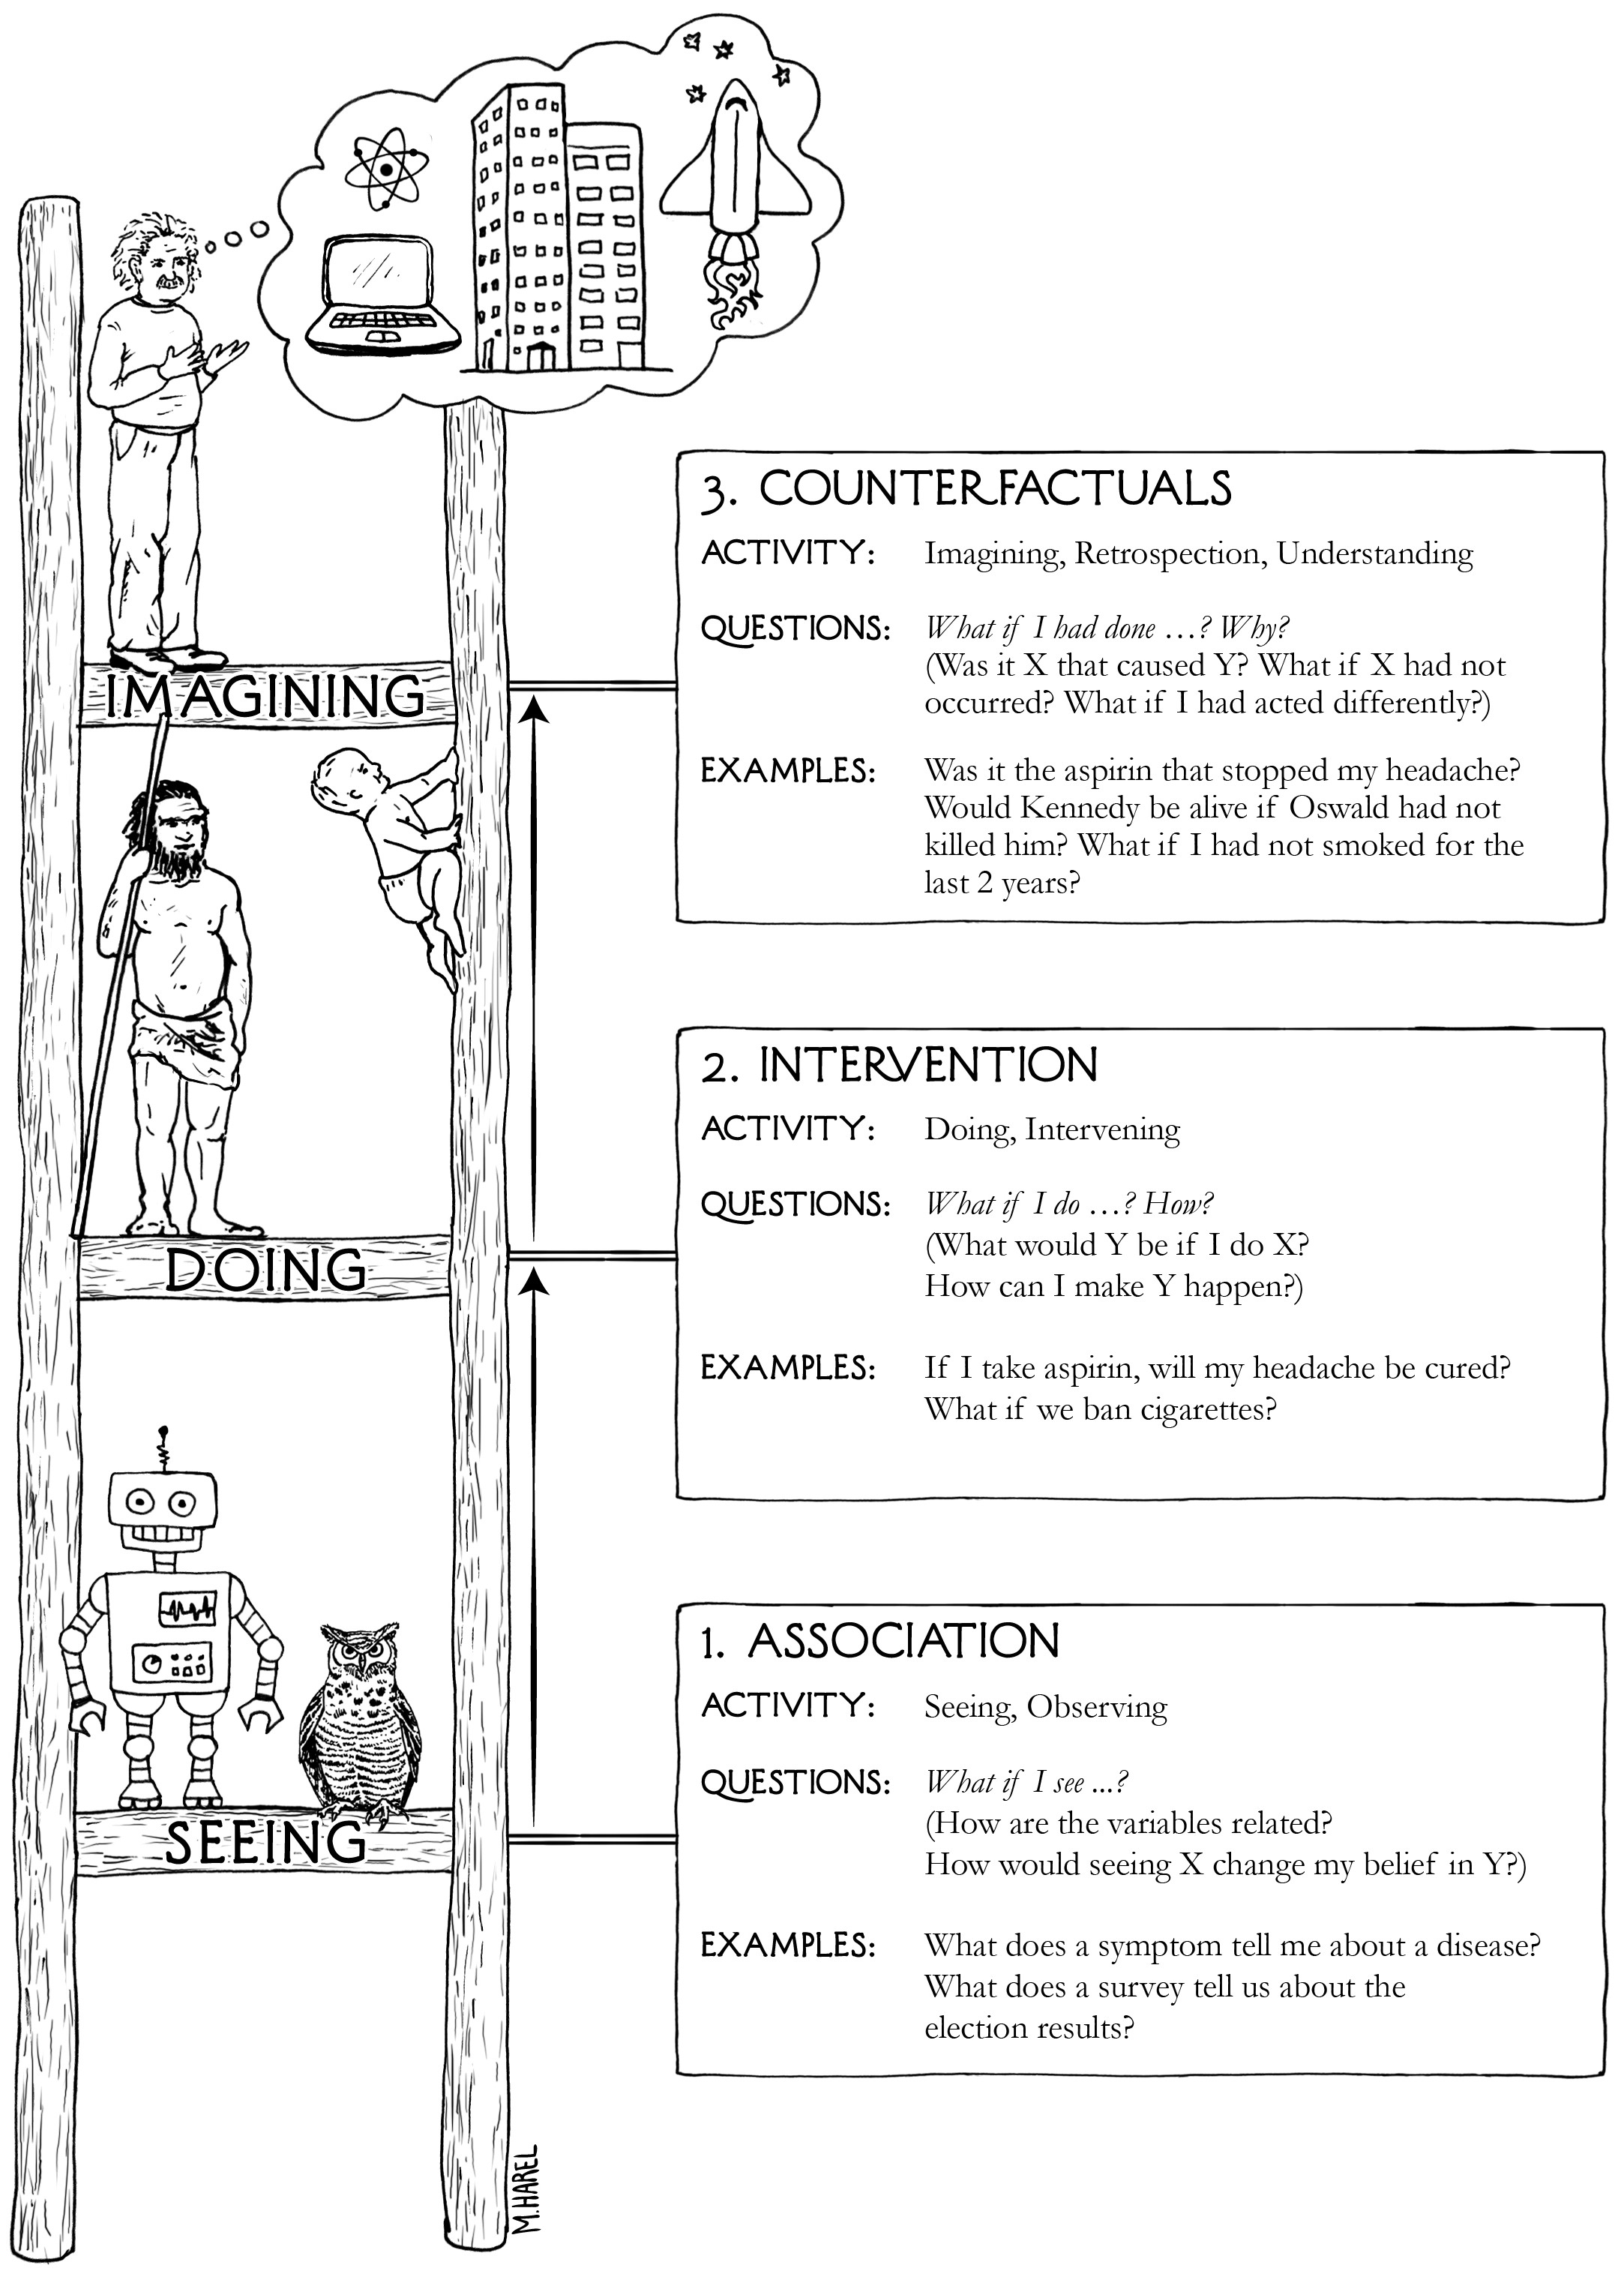
\includegraphics[width=0.45\textwidth]{ladder.jpg}};
    \draw[line width=1mm,fill=green,draw=green,->] (-4,2) -- node[below,sloped] {data-driven} (-4,-2);
    \draw[line width=1mm,fill=red,draw=red,->] (4,-2) -- node[below,sloped] {model-based} (4,2);
  \end{tikzpicture}
  \centerline{\tiny Image from Pearl \& Mackenzie, {\it The Book of Why}}
\end{frame}

\begin{frame}{Counterexample (Dawid, 2002)}
\begin{example}[1/2]
  For parameter $\rho\in[0,1]$, consider the iSCM $M^\rho$ with binary exogenous input variable $X \in \{0,1\}$, endogenous variable $Y \in \RN$, a single latent exogenous random variable $W = (W_1,W_2) \in \RN^2$ with
exogenous distribution 
  $$\begin{pmatrix} W_1 \\ W_2 \end{pmatrix}\sim\C{N}\left(\begin{pmatrix}0 \\ 0\end{pmatrix},\begin{pmatrix}1&\rho\\ \rho&1\end{pmatrix}\right)$$
and structural equation
  $$Y = W_1 (1 - X) + W_2 X.$$
  In a medical setting, this iSCM could be used to model whether a patient was treated ($x$) and the corresponding outcome for that patient ($Y^{\doit(x)}$).
\end{example}
\end{frame}

\begin{frame}{Counterexample (Dawid, 2002)}
\begin{example}[2/2]
  Suppose in the actual world, $x = 0$ and $Y^{\doit(x=0)} = y \in \RN$.
  Consider the counterfactual: {\it ``What would the outcome have been, had we assigned treatment to this patient?''}.

  Construct the twin iSCM $(M^{\rho})^{\twin}$.
  The counterfactual query then asks for $P_{(M^{\rho})^\twin}((Y')^{\doit(x'=1)}\mid Y^{\doit(x=0)}=y)$. One can calculate that
$$
  P_{(M^{\rho})^\twin}\big((Y')^{\doit(x'=1)},Y^{\doit(x=0)}\big) = \C{N}\left(\begin{pmatrix}0\\ 0\end{pmatrix}, \begin{pmatrix} 1 & \rho \\ \rho & 1 \end{pmatrix}\right)
$$
  and hence $P_{(M^{\rho})^\twin}((Y')^{\doit(x'=1)} \mid Y^{\doit(x=0)}=y) = \C{N}(\rho y,1-\rho^2)$. Note that the answer to the counterfactual query depends on a quantity $\rho$ that we cannot identify from the Markov kernel $P_{M^{\rho}}(Y\given \doit X)$, since this is independent of $\rho$. 
Indeed, iSCMs $M^{\rho}$ and $M^{\rho'}$ with $\rho\neq\rho'$ are interventionally equivalent, but not counterfactually equivalent.
%If we obtain the iSCM from a reduction, we find the one with $\rho = 1$.
\end{example}
  \textbf{Conclusion: counterfactuals cannot be inferred from data alone!}
\end{frame}



\part{Reparameterizing Latent Space}
\frame{\partpage}

\begin{frame}{Question}
  We consider exogenous random variables to be latent.
  Hence, if we reparameterize them, this may have no observable consequences.

  \begin{block}{Question}
    For which reparameterizions of the space $\CX_W$ of the exogenous random variables is the causal semantics (partially) preserved?
  \end{block}
\end{frame}

\begin{frame}{Exogenous push-forwards}
\begin{Def}[\ref{def:exogenous_pushforward}]
  Let $M = \lt J, V, W, \CX, P, f \rt$ be an iSCM.
  Let $\tilde{W}$ be a finite index set disjoint from $J \cup V \cup W$, and
  $\CX_{\tilde{W}} = \prod_{\tilde{w}\in\tilde{W}} \CX_{\tilde{w}}$ the product of standard measurable spaces $\CX_{\tilde{w}}$. 
  Let $\tilde{f} : \CXJ \times \CXV \times \CX_{\tilde{W}} \to \CXV$ and $\Phi : \CX_J \times \CX_W \to \CX_{\tilde{W}}$ be measurable mappings such that:
  \begin{enumerate}
    \item $f(x_J,x_V,x_W) = \tilde{f}(x_J,x_V,\Phi(x_J,x_W)) \quad M\as,$
    \item there exists a distribution $\tilde{P} = \bigotimes_{\tilde{w}\in\tilde{W}} \tilde{P}_{\tilde{w}}$ with $\tilde{P}_{\tilde{w}} \in \C{P}(\CX_{\tilde{w}})$ for all $\tilde{w}\in\tilde{W}$ such that
    %  $$(\id_{\CX_J}, \Phi)_* \lp \delta(X_J|X_J) \otimes P \rp = \delta(X_J|X_J) \otimes \tilde{P},$$
    %where $P = \bigotimes_{w\in W}P_w$ with $P_w \in \C{P}(\CX_w)$ for all $w \in W$.
    %$\tilde{P} := (\Phi)_* P$ factorizes as a product $\tilde{P} = \bigotimes_{\tilde{w}\in\tilde{W}} \tilde{P}_{\tilde{w}}$ of probability distributions $\tilde{P}_{\tilde{w}} \in \C{P}(\CX_{\tilde{w}})$,
    $$\forall x_J \in \CX_J: (\Phi(x_J,\cdot))_* P = \tilde{P}.$$
  \end{enumerate}
  Then we call the iSCM
  $$M_{\repar{\tilde{f}}{\Phi}} = \lt J, V, \tilde{W}, \CX_J \times \CX_V \times \CX_{\tilde{W}}, \tilde{P}, \tilde{f} \rt$$
  an \emph{exogenous push-forward} of $M$ along $\Phi$.
\end{Def}
\end{frame}

\begin{frame}{Exogenous push-forwards: properties}
Let $M = \lt J, V, W, \CX, P, f \rt$ be an iSCM, and $M_{\repar{\tilde{f}}{\Phi}} = \lt J, V, \tilde{W}, \tilde{\CX}, \tilde{P}, \tilde{f} \rt$ an exogenous push-forward of $M$.

\bigskip
Exogenous push-forwards are compatible with hard interventions.
\begin{Lem}[\ref{lem:interventions_exogenous_pushforward_commute}]
For an intervention target $T \subseteq V \cup J$:
$$(M_{\repar{\tilde{f}}{\Phi}})_{\doit(T)} = (M_{\doit(T)})_{\repar{\tilde{f}_{\sm T}}{\Phi}}.$$
\end{Lem}
The twinning operation is only compatible with exogenous push-forwards under restrictive assumptions.
\begin{Lem}[\ref{lem:twinning_exogenous_pushforward_commute}]
If $\Phi$ is constant in $X_J$, that is, $\Phi(x_J,x_W) = \Phi(\tilde{x}_J,x_W)$ for all $x_W \in \CX_W$ and all $x_J,\tilde{x}_J \in \CX_J$, then:
$$(M_{\repar{\tilde{f}}{\Phi}})^\twin = (M^\twin)_{\repar{\tilde{f}^\twin}{\Phi}}.$$
\end{Lem}
\end{frame}

\begin{frame}{Exogenous push-forwards: main result}
We can now answer the question:
\begin{Thm}[\ref{thm:various_equiv_exogenous_pushforward}]
  Let $M = \lt J, V, W, \CX, P, f \rt$ be an iSCM, and $M_{\repar{\tilde{f}}{\Phi}} = \lt J, V, \tilde{W}, \tilde{\CX}, \tilde{P}, \tilde{f} \rt$ an exogenous push-forward of $M$.

  \begin{itemize}
    \item If both $M$ and $M_{\repar{\tilde{f}}{\Phi}}$ are simple,
  then $M$ is observably and interventionally equivalent to $M_{\repar{\tilde{f}}{\Phi}}$ w.r.t.\ $V$.
    \item If, in addition, $\Phi$ does not depend on $X_J$, then $M$ is even counterfactually equivalent to $M_{\repar{\tilde{f}}{\Phi}}$ w.r.t.\ $V$.
  \end{itemize}
\end{Thm}

\bigskip
Note: Example \ref{eg:exogenous_pushforward_not_counterfactually_equivalent} shows that an exogenous push-forward need not be counterfactually equivalent w.r.t.\ $V$ if $\Phi$ depends on $X_J$.
\end{frame}

\begin{comment}
\begin{frame}{Exogenous push-forwards: proof sketch}
\begin{proof}
  Let $g : \CX_J \times \CX_W \to \CX_V$ be the solution function of $M$, 
  and $\tilde{g} : \CX_J \times \CX_{\tilde{W}} \to \CX_V$ the solution function of $\tilde{M} := M_{\repar{\tilde{f}}{\Phi}}$.
  The first step is to show that
  $$g = \tilde g \circ (\id_{\CX_J},\Phi).$$

  From Theorem~\ref{thm:scm_unique_solvability} it then follows that
  $P_{M}(X_V \mid \doit(X_J)) = P_{M_{\repar{\tilde{f}}{\Phi}}}(X_V \mid \doit(X_J))$, which shows
  the observable equivalence w.r.t.\ $V$.
  
  With the help of Lemma~\ref{lem:interventions_exogenous_pushforward_commute} this implies that
  $M$ and $M_{\repar{\tilde{f}}{\Phi}}$ are interventionally equivalent w.r.t.\ $V$.

  Assume now that $\Phi$ does not depend on $X_J$. By Lemma~\ref{lem:twinning_exogenous_pushforward_commute}, 
  $(M_{\repar{\tilde{f}}{\Phi}})^\twin = (M^\twin)_{\repar{\tilde{f}^\twin}{\Phi}}$.
  The interventional equivalence of $M^\twin$ and its exogenous push-forward $(M^\twin)_{\repar{\tilde{f}^\twin}{\Phi}}$ w.r.t.\ $V \cup V'$ then implies the counterfactual equivalence w.r.t.\ $V$ of $M$ and $M_{\repar{\tilde{f}}{\Phi}}$.
\end{proof}
\end{frame}

\begin{frame}{Corollary for special case}
A special case of interest is obtained for `pointwise' surjective mappings $\Phi$.
\begin{Cor}
  If $x_W \mapsto \Phi(x_J,x_W)$ is surjective for all $x_J \in \CX_J$, then unique solvability of $M$ implies unique solvability of $M_{\repar{\tilde{f}}{\Phi}}$,
%  and unique solvability of $M_{\doit(T)}$ implies unique solvability of $(M_{\repar{\tilde{f}}{\Phi}})_{\doit(T)}$ for any $T \subseteq V \cup J$.
  and simplicity of $M$ implies simplicity of $M_{\repar{\tilde{f}}{\Phi}}$.
\end{Cor}
\end{frame}

\begin{frame}{Example 1}
\begin{Eg}[\ref{eg:merging_exogenous_random_variables}: Merging exogenous random variables]
  Let $M = \lt J, V, W, \CX, P, f \rt$ be an iSCM.
  Let $\tilde{W}$ be a partition of $W$.
  Take for $\CX_{\tilde{W}} = \prod_{\tilde{w}\in\tilde{W}} \CX_{\tilde{w}}$ the product of standard measurable spaces $\CX_{\tilde{w}} = \prod_{w \in \tilde{w}} \CX_w$. 
  Let $\Phi : \CX_W \to \CX_{\tilde{W}}$ be the natural identification that
  maps $x_W = (x_w)_{w\in W} \in \CX_W$ with components $x_w \in \CX_w$ to $x_{\tilde{W}} = (x_{\tilde{w}})_{\tilde{w}\in\tilde{W}} \in \CX_{\tilde{W}}$ with components $x_{\tilde{w}} = (x_w)_{w \in \tilde{w}} \in \CX_{\tilde{w}}$.
  Because $\tilde{W}$ is a partition of $W$, $\Phi$ is a bijection.
  Take
  $$\tilde{f} : \CXJ \times \CXV \times \CX_{\tilde{W}} \to \CXV : (x_J,x_V,x_{\tilde{W}}) \mapsto f(x_J,x_V,\Phi^{-1}(x_{\tilde{W}})).$$
  It is immediate from Definition~\ref{def:exogenous_pushforward} that 
  $$M_{\repar{\tilde{f}}{\Phi}} = \lt J, V, \tilde{W}, \CX_J \times \CX_V \times \CX_{\tilde{W}}, \tilde{P}, \tilde{f} \rt$$
  is an exogenous push-forward of $M$.
  Because $\Phi$ is independent of $x_J$ and bijective, $M_{\repar{\tilde{f}}{\Phi}}$ is observably, interventionally and counterfactually equivalent to $M$ w.r.t.\ $V$ in case $M$ is simple.
\end{Eg}
\end{frame}
\end{comment}

\begin{frame}{Example}
%The following example shows that an exogenous pushforward need not be counterfactually equivalent w.r.t.\ $V$ if $\Phi$ depends on $X_J$.
\begin{Eg}[\ref{eg:exogenous_pushforward_not_counterfactually_equivalent}]
Consider the acyclic iSCM $M$ with exogenous input variable $X_1$ with co-domain $\{-1,1\}$, endogenous variables $X_2,X_3$ with co-domains $\{-1,1\}$, $\{-2,0,2\}$, respectively, and causal mechanism
  $$\begin{aligned} 
    X_2 &= f_2(X_1,X_B) = X_1 X_B \\
    X_3 &= f_3(X_2,X_B) = X_2 + X_B,
  \end{aligned}$$
with exogenous random variable $X_B \sim \mathrm{Uni}(\{-1,1\})$.
Consider the exogenous push-forward $\tilde{M}$ with exogenous random variable $X_{\tilde{B}}$ with co-domain $\{-1,1\}$, mapping $\Phi : \{-1,1\}^2 \to \{-1,1\} : (x_1,x_B) \mapsto x_1 x_B$, and causal mechanism
  $$\begin{aligned} 
    X_2 &= \tilde{f}_2(X_{\tilde{B}}) = X_{\tilde{B}} \\
    X_3 &= \tilde{f}_3(X_1, X_2, X_{\tilde{B}}) = X_2 + X_1 X_{\tilde{B}}.
  \end{aligned}$$ 
\end{Eg}
\end{frame}

\begin{frame}{Example 2, continued}
  \begin{Exc}
Check that this gives an exogenous push-forward (what is $\Prb(X_{\tilde{B}})$)?
  \end{Exc}
  \pause
\begin{Eg}[\ref{eg:exogenous_pushforward_not_counterfactually_equivalent}, continued]
$\Prb(X_{\tilde{B}}) = \Phi_*(\Prb(X_B)) = \mathrm{Uni}(\{-1,1\})$.
Also, $\tilde{f}$ and $\Phi$ satisfy the requirement for a exogenous push-forward:
  $$\begin{aligned}
    \tilde{f}(x_1,x_2,\Phi(x_1,x_B)) 
    &= (\Phi(x_1,x_B), x_2 + x_1 \Phi(x_1,x_B)) \\
    &= (x_1 x_B, x_2 + x_1 x_1 x_B) \\
    &= (x_1 x_B, x_2 + x_B) \\
    &= f(x_1,x_2,x_B).
  \end{aligned}$$
Both $M$ and $\tilde{M}$ are acyclic, hence simple.

By Theorem~\ref{thm:various_equiv_exogenous_pushforward}, $\tilde{M}$ is observably and interventionally equivalent to $M$ w.r.t.\ $\{X_2,X_3\}$.
However, $\tilde{M}$ is not counterfactually equivalent to $M$ w.r.t.\ $\{X_2,X_3\}$, as one can check explicitly (do this!).
%The causal mechanism of $M^\twin$ is:
%  $$\begin{aligned} 
%    X_2 &= f_2(X_1,X_B) = X_1 X_B \\
%    X_3 &= f_3(X_2,X_B) = X_2 + X_B \\
%    X_{2'} &= f_2(X_{1'},X_B) = X_{1'} X_B \\
%    X_{3'} &= f_3(X_{2'},X_B) = X_{2'} + X_B,
%  \end{aligned}$$ 
%while that of $\tilde{M}^\twin$ is:
%  $$\begin{aligned} 
%    X_2 &= \tilde{f}_2(X_{\tilde{B}}) = X_{\tilde{B}} \\
%    X_3 &= \tilde{f}_3(X_1, X_2, X_{\tilde{B}}) = X_2 + X_1 X_{\tilde{B}} \\
%    X_{2'} &= \tilde{f}_2(X_{\tilde{B}}) = X_{\tilde{B}} \\
%    X_{3'} &= \tilde{f}_3(X_{1'}, X_{2'}, X_{\tilde{B}}) = X_{2'} + X_{1'} X_{\tilde{B}},
%  \end{aligned}$$ 
%The observation $X_1 = 1$, $X_2 = 1$ implies $X_B = 1$ and $X_3 = 2$ in $M$, whereas it implies $X_{\tilde{B}} = 1$ and $X_3=2$ in $\tilde{M}$.
%If we do $X_{1'} = -1$, this results in $X_{2'} = -1$, $X_{3'} = 0$ in $M$, and in $X_{2'} = 1$, $X_{3'} = 0$ in $\tilde{M}$.
%$M$ and $\tilde{M}$ are clearly not counterfactually equivalent with respect to $\{2,3\}$ (even not with respect to $\{2\}$ only)!
\end{Eg}
\end{frame}

\part{Response functions}
\frame{\partpage}

\begin{frame}{Response functions (Balke \& Pearl, 1994)}
  \begin{itemize}
    \item \emph{Response functions} can be used to parameterize iSCMs.
    \item We give an example rather than a general treatment.
  \end{itemize}

\begin{Def}[\ref{def:response_functions}]
  Let $M = \lt J, V=\{v\}, W, \CX_J \times \CX_V \times \CX_W, P, f \rt$ be a simple iSCM
  with $\C{X}_J$ and $\C{X}_v$ both discrete (and $\C{X}_W$ arbitrary).
  \begin{itemize}
    \item Let $\tilde{W}:=\{\tilde{w}\}$ be a singleton; consider the space of measurable functions
      $\C{X}_{\tilde{W}} = (\C{X}_v)^{\C{X}_J} = \{\phi : \C{X}_J \to \C{X}_v\}$
      (called ``response functions'' \cite{BalkePearl1994b}).
  \item $M$ defines a function $\Phi : \C{X}_W \to \C{X}_{\tilde{w}}$ that assigns to each $x_w \in \C{X}_w$ the corresponding response function in $\C{X}_{\tilde{W}}$:
  $\Phi(x_W) : x_J \mapsto f_v(x_J, x_W)$.
\item We call $M_{\repar{\tilde{f}}{\Phi}} := \lt J, V=\{v\}, \tilde{W}, \CX_J \times \CX_V \times \C{X}_{\tilde{W}}, \tilde{P}, \tilde{f} \rp$,
    \begin{itemize}
      \item with exogenous distribution $\tilde{P} = (\Phi)_* (P)$,
      \item and causal mechanism $\tilde{f}(x_J,x_{\tilde{W}}) = x_{\tilde{W}}(x_J)$\\
        (which just evaluates the response function $x_{\tilde{W}}$ in the input $x_J$).
    \end{itemize}
    the \emph{response variable parameterization} of $M$.
  \end{itemize}
  \end{Def}
\end{frame}

\begin{comment}
\begin{frame}{Response functions, continued}
\begin{Prp}[\ref{prp:counterfactual_equivalence_response_functions}]
  $\tilde{M}$ in Definition~\ref{def:response_functions} is counterfactually equivalent to $M$ w.r.t.\ $V$.
\end{Prp}
\begin{block}{Proof}
\setlength\abovedisplayskip{5pt}
\setlength\belowdisplayskip{5pt}
%  Note that:
%    $$f_v(x_j,x_w) = \Phi_w(x_w)(x_j) = \tilde{f}_v(x_j,\Phi_w(x_w))$$
%  for all $x_j \in \CX_j, x_w \in \CX_w$.
%  Hence, by Theorem~\ref{thm:scm_unique_solvability}, 
%  \begin{align*}
%    P_{M}(X_v \mid \doit(X_j)) & = (f_v)_* \lp \delta(X_j|X_j) \otimes P(X_w) \rp \\
%    & = (\tilde{f}_v)_* \lp \delta(X_j|X_j) \otimes (\Phi_w)_* P(X_w) \rp \\
%    & = (\tilde{f}_v)_* \lp \delta(X_j|X_j) \otimes \tilde{P}(\tilde{X}_w)  \rp \\
%    & = P_{\tilde{M}}(X_v \mid \doit(X_j)).
%  \end{align*}
%
%  It is obvious that a hard intervention targeting $\{v\}$ will lead to the same intervened Markov kernel in both iSCMs.
%  Hence they are interventionally equivalent w.r.t.\ $V$.
%
  Consider $M^\twin$ and $\tilde{M}^\twin$.
  The causal mechanism of $M^\twin$ is given by:
  $$\begin{cases}
    f^\twin_v(x_j,x_{j'},x_w) = f_v(x_j,x_w), \\
    f^\twin_{v'}(x_j,x_{j'},x_w) = f_v(x_{j'},x_w)
  \end{cases}$$
  for $x_j, x_{j'} \in \CX_j$ and $x_w \in \CX_w$, while that of $\tilde{M}^\twin$ satifies:
  $$\begin{cases}
    \tilde{f}^\twin_v(x_j,x_{j'},\tilde{x}_w) = \tilde{f}_v(x_j,\tilde{x}_w) = \tilde{x}_w(x_j), \\
    \tilde{f}^\twin_{v'}(x_j,x_{j'},\tilde{x}_w) = \tilde{f}_v(x_{j'},\tilde{x}_w) = \tilde{x}_w(x_{j'})
  \end{cases}$$
  for $x_j, x_{j'} \in \CX_j$ and $x_{\tilde{w}} \in \CX_{\tilde{w}}$. 
  Hence, for all  for $x_j, x_{j'} \in \CX_j$ and $x_w \in \CX_w$:
  $$\begin{cases}
    \tilde{f}^\twin_v(x_j,x_{j'},\Phi_w(x_w)) = \tilde{f}_v(x_j,\Phi_w(x_w)) = f_v(x_j,x_w) = f^\twin_v(x_j,x_{j'},x_w), \\
    \tilde{f}^\twin_{v'}(x_j,x_{j'},\Phi_w(x_w)) = \tilde{f}_v(x_{j'},\Phi_w(x_w)) = f_v(x_{j'},x_w) = f^\twin_{v'}(x_j,x_{j'},x_w).
  \end{cases}$$
\end{block}
\end{frame}

\begin{frame}{Response functions, continued}
  \begin{proof}[Proof (continued)]
  Writing this more compactly:
  $$\tilde{f}^\twin_v(x_j,x_{j'},\Phi_w(x_w)) = f^\twin(x_j,x_{j'},x_w).$$
  Hence, by Theorem~\ref{thm:scm_unique_solvability}: 
  \begin{align*}
    P_{M^\twin}(X_v,X_{v'} \mid \doit(X_j,X_{j'})) & = (f^\twin)_* \lp \delta(X_j,X_{j'}|X_j,X_{j'}) \otimes P(X_w)\rp \\
    & = (\tilde{f}^\twin)_* \lp \delta(X_j,X_{j'}|X_j,X_{j'}) \otimes (\Phi_w)_* P(X_w) \rp \\
    & = (\tilde{f}^\twin)_* \lp \delta(X_j,X_{j'}|X_j,X_{j'}) \otimes \tilde{P}(\tilde{X}_w) \rp \\
    & = P_{\tilde{M}^\twin}(X_v,X_{v'} \mid \doit(X_j,X_{j'})).
  \end{align*}
  It is obvious that a hard intervention targeting any subset of $\{v,v'\}$ will lead to the same intervened Markov kernel in $M^\twin$ and $\tilde{M}^\twin$.
  Hence $M^\twin$ and $\tilde{M}^\twin$ are interventionally equivalent w.r.t.\ $V \cup V'$, which shows that $M$ and $\tilde{M}$ are counterfactually equivalent w.r.t.\ $V$.
\end{proof}
\end{frame}
\end{comment}

\begin{frame}{Response functions, continued}
We call it a parameterization because it preserves the important causal semantics:
\begin{Prp}[\ref{prp:counterfactual_equivalence_response_functions}]
  The response variable parameterization of $M$ in Definition~\ref{def:response_functions} is an exogenous push-forward of $M$ and is counterfactually equivalent to $M$ w.r.t.\ $V$.
\end{Prp}
\begin{proof}
  Note that:
    $$f(x_J,x_W) = \Phi(x_W)(x_J) = \tilde{f}(x_J,\Phi(x_W))$$
  for all $x_J \in \CX_J, x_W \in \CX_W$.
  Because $M$ and $\tilde{M}$ are both acyclic, they are both simple, and the claim now follows from Theorem~\ref{thm:various_equiv_exogenous_pushforward}, noting that $\Phi$ does not depend on $X_J$.
\end{proof}
\end{frame}


\begin{frame}{Response functions, continued}
\begin{Cor}[\ref{cor:counterfactual_equivalence_response_functions}]
  Let $M = \lt J, V, W, \CX, P, f \rt$ be a simple iSCM with discrete exogenous input space $\CX_J$.
  Let $v \in V$ be an endogenous variable in $M$ taking values in a discrete space $\CX_v$.
  Then there exists an iSCM that is counterfactually equivalent to $M$ w.r.t.\ $\{v\}$ that has
  just a single endogenous variable ($V=\{v\}$ with space $\CX_v$) and exogenous random space $(\CX_v)^{\CX_J}$.
\end{Cor}
\begin{proof}
  First marginalize out all endogenous variables except $v$, and then take the response variable parameterization of this marginal iSCM.
%  Marginalize out all endogenous variables except $v$:
%  $$M_v := (M)_{\sm (V\sm v)} = \lt J, \{v\}, W, \CX_J \times \CX_v \times \CX_W, P, f_{\sm} \rt.$$
%  Now use Definition~\ref{def:response_functions} to construct the response function parameterization
%  $$\tilde{M} := (M_v)_{\repar{\widetilde{f_{\sm}}}{\Phi}}.$$
  It has the desired exogenous random space, and note that both operations preserve counterfactual equivalence w.r.t.\ $\{v\}$.
\end{proof}
\end{frame}

\part{Bounding counterfactuals}
\frame{\partpage}

\begin{frame}{Application: bounding counterfactuals}
  \begin{itemize}
    \item Estimating counterfactual probabilities from data can be impossible without relying on very strong modeling assumptions.
    \item We can sometimes derive a \emph{bound} on counterfactual probabilities \cite{BalkePearl1994b}.
    \item One way to derive such bounds on counterfactuals exploits the response function parameterization.
  \end{itemize}

  \bigskip
  \begin{block}{Motivation}
    Joe participated in a randomized controlled trial. He was assigned to the placebo group, and was not cured.
    His physician asks: would Joe have been cured if he had been assigned to the treatment group?
  \end{block}
\end{frame}

\begin{frame}{Application: bounding counterfactuals}
\begin{Prp}[\ref{prp:Bounding_counterfactuals}, Bounding counterfactual probabilities]
  For a simple iSCM $M$ with a single binary exogenous input variable $X \in \{0,1\}$ and a binary endogenous variable $Y \in \{0,1\}$
  (and possibly additional endogenous variables and exogenous random variables), the counterfactual probability
  $$P_{M^{\twin}}\big((Y')^{\doit(x'=1)}=1\mid Y^{\doit(x=0)}=0\big)$$
  (with $Y^{\doit(x=0)}$ the factual outcome, and $(Y')^{\doit(x'=1)}$ the counterfactual outcome)
  is bounded by:
  {\small\begin{equation*}
    \frac{q_{0|0} - \min(q_{0|0},q_{0|1})}{q_{0|0}} 
    \le P_{M^\twin}((Y')^{\doit(x'=1)} = 1 | Y^{\doit(x=0)}=0)
    \le \frac{\min(q_{0|0},q_{1|1})}{q_{0|0}},
  \end{equation*}}
  where $q_{y|x} := P_M(Y=y\given \doit(X=x))$.
\end{Prp}
\end{frame}

\begin{frame}{Bounding counterfactuals (proof)}
  \begin{block}{Proof}
    Denote the $3$-dimensional probability simplex by $\Delta_3=\{r=(r_{00},r_{01},r_{10},r_{11}) \in [0,1]^4 : r_{00}+r_{01}+r_{10}+r_{11}= 1\}$.
  
    By Corollary~\ref{cor:counterfactual_equivalence_response_functions}, we may without loss of generality assume that the iSCM has only a single binary endogenous variable $Y$ and an exogenous random variable taking values in $\{0,1\}^{\{0,1\}}$.

    That iSCM must then be a member of the family $\{M^\rho : \rho \in \Delta_3\}$, where the iSCM $M^\rho$ with parameter $\rho$ has binary exogenous input variable $X$, binary endogenous variable $Y$, a single latent exogenous random variable $W \in \{f_{00},f_{01},f_{10},f_{11}\}$, exogenous distribution $P^\rho(W=f_w) = \rho_w$, and structural equation
  $Y^{\doit(x)} = W(x),$
where we defined response functions $f_{00},f_{01},f_{10},f_{11} : \{0,1\} \to \{0,1\}$ by:
    {\small\begin{align*}
    f_{00} &: 0 \mapsto 0, 1 \mapsto 0;\\
    f_{01} &: 0 \mapsto 0, 1 \mapsto 1;\\
    f_{10} &: 0 \mapsto 1, 1 \mapsto 0;\\
    f_{11} &: 0 \mapsto 1, 1 \mapsto 1.
    \end{align*}}
  \end{block}{Proof}
\end{frame}


\begin{frame}{Bounding counterfactuals (proof, continued)}
  \begin{block}{Proof}
  We will derive a bound on the counterfactual probability
    $$P_{(M^{\rho})^{\twin}}((Y')^{\doit(x'=1)}=1\mid Y^{\doit(x=0)}=0).$$
    \vskip-0.5\baselineskip
    \begin{description}
      \item[Abduction] Update the exogenous distribution with the factual outcome.
        {\small
        $$P_{(M^{\rho})^{\twin}}(W=w | Y^{\doit(x=0)}=0) = 
    \begin{cases}
      \frac{\rho_{00}}{\rho_{00} + \rho_{01}} & w = f_{00}, \\
      \frac{\rho_{01}}{\rho_{00} + \rho_{01}} & w = f_{01}, \\
      0 & w = f_{10}, \\
      0 & w = f_{11}.
    \end{cases}$$}
  \item[Prediction] Predict the counterfactual outcome, using the updated distribution of $W$.
    We can calculate:
        $$P_{(M^{\rho})^\twin}((Y')^{\doit(x'=1)} = 1 | Y^{\doit(x=0)}=0) = \frac{\rho_{01}}{\rho_{00} + \rho_{01}}.$$
    \end{description}
  \end{block}
\end{frame}

\begin{frame}{Bounding counterfactuals (proof, continued)}
  \begin{block}{Proof}
Because of the counterfactual equivalence of $M^\rho$ and $M$ w.r.t.\ $Y$, we have that
  $q_{y|x} := P_M(Y=y\given \doit(X=x)) = P_{(M^{\rho})^\twin}(Y=y\given \doit(X=x))$.
This Markov kernel is given explicitly by:\\
  \smallskip
  \centerline{\small\begin{tabular}{ccl}
    $x$ & $y$ & $q_{y|x}$ \\
    \hline
    0   & 0   & $\rho_{00} + \rho_{01}$ \\ % = 1-eps
    0   & 1   & $\rho_{10} + \rho_{11}$ \\ %= eps
    1   & 0   & $\rho_{00} + \rho_{10}$ \\ %= delta
    1   & 1   & $\rho_{01} + \rho_{11}$ \\ %= 1-delta
    \end{tabular}}

    \bigskip
For our particular counterfactual probability of interest, we get
  $$P_{(M^{\rho})^\twin}((Y')^{\doit(x'=1)} = 1 | Y^{\doit(x=0)}=0) = \frac{\rho_{01}}{q_{0|0}}.$$
  \end{block}
\end{frame}

\begin{frame}{Bounding counterfactuals (proof, continued)}
  \begin{proof}
From the non-negativity of the $\rho$'s and the table above, we can derive the bound
$$q_{0|0} - \min(q_{0|0},q_{0|1}) \le \rho_{01} \le \min(q_{0|0},q_{1|1})$$
and hence
{\small $$\frac{q_{0|0} - \min(q_{0|0},q_{0|1})}{q_{0|0}} \le P_{(M^{\rho})^\twin}((Y')^{\doit(x'=1)} = 1 | Y^{\doit(x=0)}=0) \le \frac{\min(q_{0|0},q_{1|1})}{q_{0|0}}$$}

Since $M^\rho$ is counterfactually equivalent to the original iSCM $M$ w.r.t.\ $Y$, the same bound also holds for $M$ itself.
  \end{proof}

\bigskip 
Example: in the almost-deterministic case ($q_{0|0} \approx 1$ and $q_{1|1} \approx 1$),
  the bound tells us that $P_{(M^{\rho})^\twin}((Y')^{\doit(x'=1)} = 1 | Y^{\doit(x=0)}=0) \approx 1$.
\end{frame}

\end{document}

\part{Causal Discovery: Faithfulness}
\frame{\partpage}

\begin{frame}{Faithfulness}
A simple iSCM is called $\sigma$-faithful ($d$-faithful) if each conditional independence in its Markov kernel
is due to a $\sigma$-separation ($d$-separation).
\begin{Def}[\ref{def:faithfulness}]
  Let $M = \lt \Sin, \Send, \Srnd, \CX, P, f \rt$ be a simple iSCM with graph $G(M)$
  and Markov kernel $P_{M}(X_V \given \doit(X_J))$.
  $M$ is called \emph{$\sigma$-faithful} if 
  for all $A, B, C \ins J \cup V$:
  \begin{equation}\label{slides:eq:sigma_faithful}
    A \Perp^\sigma_{G(M)} B \given C \impliedby X_A \Indep_{P_{M}(X_V \given \doit(\XJ))} X_B \given X_C.
  \end{equation}
  It is called \emph{$d$-faithful} if
  for all $A, B, C \ins J \cup V$:
  \begin{equation*}
    A \Perp^d_{G(M)} B \given C \impliedby X_A \Indep_{P_{M}(X_V \given \doit(\XJ))} X_B \given X_C.
  \end{equation*}
%  If one wants to make the implicit dependence on $J$ more explicit one can equivalently also write:
%  $$A \Perp^\sigma_{G(M)} J \cup B \given C \impliedby X_A \Indep_{P_{M}(X_V,X_W \given \doit(\XJ))} X_J,X_B \given X_C.$$
  For a subset $O \subseteq V$, we say that $M$ is \emph{$\sigma$-faithful w.r.t.\ $O$} if
  \eref{slides:eq:sigma_faithful} holds for all $A, B, C \ins J \cup O$, and define
  \emph{$d$-faithful w.r.t.\ $O$} analogously.
\end{Def}
\end{frame}

\begin{frame}{Faithfulness Violations}
These definitions behave properly under marginalization:
\begin{Rem}
A simple iSCM $M$ is $\sigma$/$d$-faithful w.r.t.\ $O$ if and only if
its marginalization $M_O$ is $\sigma$/$d$-faithful.
\end{Rem}

\bigskip
Faithfulness may fail for various reasons:
\begin{itemize}
  \item Deterministic relationships may lead to additional conditional independences, but are not exploited by the Markov property;
  \item Effects may cancel out;
  \item If cycles are present, and (i) all variables are discrete, or (ii) interactions are linear;
  \item If cycles are present, and the system is ``perfectly adapting''.
\end{itemize}
\end{frame}

\begin{frame}{Faithfulness Violation Examples}
\begin{Eg}[Determinism]
  Take an iSCM with three endogenous variables $X,Y,Z$ and two exogenous random variables $U,W$, with structural equations
  $$X = 5, \qquad Y = X + U, \qquad Z = X + W.$$
  Then $Y \nPerp Z$ but $Y \Indep Z$.
  This simple (even acyclic) iSCM is not faithful due to $X$ being constant.
\end{Eg}

\begin{Eg}[Canceling Effects]
  Take an iSCM with three endogenous variables $X,Y,Z$ and three exogenous random variables $W_X,W_Y,W_Z$, with structural equations
  $$X = W_X, \qquad Y = X + W_Y, \qquad Z = Y - X + W_Z.$$
  Then $X \nPerp Z$ but $X \Indep Z$.
\end{Eg}
\end{frame}

\begin{frame}{$\sigma$-Faithfulness Violation}
One can show that in certain special cases, the global Markov property in terms of $d$-separation even holds for simple iSCMs.
\begin{Prp}[\ref{prp:when_d-separation_holds}]
  Let $M = \lt \Sin, \Send, \Srnd, \CX, P, f \rt$ be a simple iSCM with causal graph $G(M)$ and Markov kernel $P_{M}(X_V \given \doit(X_J))$.
  If $J = \emptyset$ and one of the three conditions applies:
  \begin{enumerate}
    \item all spaces $\CX_v$ with $v \in V$ are discrete, or
    \item $M$ is essentially linear over $\RN$ and the transformed exogenous distribution has a density w.r.t.\ Lebesgue measure, or
    \item $M$ is acyclic,
  \end{enumerate} 
  then for all $A, B, C \ins J \cup V$:
  $$A \Perp^d_{G(M)} B \given C \implies X_A \Indep_{P_{M}(X_V \given \doit(\XJ))} X_B \given X_C.$$
\end{Prp}
\end{frame}


\part{Causal Discovery: The Basics}
\frame{\partpage}

\begin{frame}{Outline}
  We give mathematical definitions for:
  \begin{itemize}
    \item $a$ causes $b$;
    \item $a$ is a direct cause of $b$;
    \item $a$ and $b$ have a common cause
  \end{itemize}
  and relate this to properties of the (intervened) Markov kernels.

  \medskip
  We then study three causal discovery methods:
  \begin{enumerate}
    \item Randomized Controlled Trials
    \item Local Causal Discovery
    \item Y-structures
  \end{enumerate}

  \bigskip
  In the following slides, we always assume that
  $M = \lt \Sin, \Send, \Srnd, \CX, P, f \rt$ is a simple iSCM with graph $G = G(M)$.

  \bigskip
  For L-CBNs, everything can be done analogously.
\end{frame}

\begin{frame}{Defining Causal Relations}\label{frame:causes}
\begin{Def}[\ref{def:cause_of}]
  If $a \in \Anc^G(b)\sm \{b\}$ for $a, b \in J \cup V \cup W$ we say that \emph{$a$ is a cause of $b$ according to $M$}.
\end{Def}
Only if $a$ causes $b$ according to $M$, a hard intervention on $a$ can change the distribution of $b$: 
\begin{Prp}[\ref{prp:scm_causes_separation}]
  Let $a \in V \cup W \cup J$ and $b \in V$. Suppose that $a \notin \Anc^{G(M)}(b)$.
  $$\begin{cases}
    \text{If } a \in V \cup W & \text{then\quad} P_{M}(X_b \given \doit(X_J), \doit(X_a)) = P_{M}(X_b \given \doit(X_J)) \\
    \text{If } a \in J        & \text{then\quad} P_{M}(X_b \given \doit(X_J)) = P_{M}(X_b \given \doit(X_{J\setminus \{a\}}),\cancel{\doit(X_a)}).
  \end{cases}$$
  Note: both cases can also be combined into a single statement:
    $$a \notin \Anc^{G(M)}(b) \implies P_{M}(X_b \given \doit(X_{J \cup \{a\}}) = P_{M}(X_b \given \doit(X_{J\sm\{a\}})).$$
\end{Prp}
Proof: Application of rules 3 and 4 of the do-calculus.
\end{frame}

\begin{frame}{Detecting Causal Relations}
This leads to a practical way of detecting the presence of a causal relation.
  \begin{Cor}[\ref{cor:scm_identify_causal_relation}]
  Let $b \in V$.
  For $a \in V \cup W \cup J$ with $a \ne b$, if
  there exist $x_{J\sm\{a\}} \in \CX_{J\sm\{a\}}$, $x_a,x_a' \in \CX_a$ such that
      \begin{equation*}\begin{split}
        & P_{M}(X_b \given \doit(X_a=x_a),\doit(X_{J\setminus \{a\}}=x_{J\setminus \{a\}})) \\
        {} \ne {} & P_{M}(X_b \given \doit(X_a=x_a'),\doit(X_{J\setminus\{a\}}=x_{J\setminus\{a\}})),
      \end{split}\end{equation*}
  then $a$ is a cause of $b$ according to $M$, that is, $a \in \Anc^{G(M)}(b)$.

  Also, for $a \in V \cup W$ with $a \ne b$, if
  there exist $x_J \in \CX_J$, $x_a \in \CX_a$ such that
  $$P_{M}(X_b \given \doit(X_a=x_a),\doit(X_J=x_J)) \ne P_{M}(X_b \given \doit(X_J=x_J)),$$
  then $a$ is a cause of $b$ according to $M$.  
\end{Cor}
\end{frame}

\begin{frame}{Defining Direct Causal Relations}
The notion of direct causation is always relative to some set of variables.
\begin{Def}[\ref{def:direct_cause_of}]
  If $a \in \Pa^{G(M)}(b)$ for $a, b \in J \cup V \cup W$ with $a\ne b$ we say that \emph{$a$ is a direct cause of $b$ w.r.t.\ $V \cup W \cup J$ according to $M$}.
\end{Def}
This property is not necessarily preserved under marginalization!

\bigskip
Direct causation can be expressed in terms of causation in an intervened iSCM:
\begin{Prp}[\ref{prp:direct_cause_of}]
  For $a,b \in J \cup V \cup W$, $a$ is a direct cause of $b$ w.r.t.\ $J \cup V \cup W$ according to $M$ if and only if $a$ is a cause of $b$ according to $M_{\doit((V \cup W \sm \{b\})}$.
\end{Prp}

\end{frame}

\begin{frame}{Detecting Direct Causal Relations}
\begin{Cor}[\ref{cor:scm_identify_direct_causal_relation}]
  Let $b \in V$.
  For $a \in V \cup W \cup J$ with $a \ne b$, if there exist $x_{J\setminus\{a\}} \in \CX_{J\sm\{a\}}$, $x_{V\setminus\{a,b\}} \in \CX_{V\setminus\{a,b\}}$, $x_a,x_a' \in \CX_a$ such that
      \begin{equation*}\begin{split}
        & P_{M}(X_b \given \doit(X_a=x_a),\doit(X_{V\setminus\{a,b\}}=x_{V\setminus\{a,b\}}),\doit(X_{J\setminus \{a\}}=x_{J\setminus \{a\}})) \\
        {} \ne {} & P_{M}(X_b \given \doit(X_a=x_a'),\doit(X_{V\setminus\{a,b\}}=x_{V\setminus\{a,b\}}),\doit(X_{J\setminus\{a\}}=x_{J\setminus\{a\}})),
      \end{split}\end{equation*}
  then $a$ is a direct cause of $b$ w.r.t.\ $V \cup J \cup W$ according to $M$.

  Also, for $a \in V \cup W$ with $a \ne b$, if there exist $x_J \in \CX_J$, $x_{V\setminus\{a,b\}} \in \CX_{V\setminus\{a,b\}}$, $x_a \in \CX_a$ such that
      \begin{equation*}\begin{split}
        & P_{M}(X_b \given \doit(X_a=x_a),\doit(X_{V\setminus\{a,b\}}=x_{V\setminus\{a,b\}}),\doit(X_J=x_J)) \\
        {} \ne {} & P_{M}(X_b \given \doit(X_{V\setminus\{a,b\}}=x_{V\setminus\{a,b\}}),\doit(X_J=x_J)),
      \end{split}\end{equation*}
  then $a$ is a direct cause of $b$ w.r.t.\ $V \cup J \cup W$ according to $M$.
  
  Thus in both cases, $a \in \Pa^{G(M)}(b)$.
\end{Cor}
\end{frame}

\begin{frame}{Bifurcations}
  \begin{Def}
    Let $G = \lt J, V, E, L \rt$ be a CDMG. 
    A \emph{bifurcation} from $v$ to $w$ in $G$ is a walk of the form:
        \[v=v_0 \hut v_1 \hut  \cdots \hut v_{k-1} \hus v_k  \tuh \cdots \tuh v_{n-1} \tuh v_n=w,\]
   %             \[v=v_0 \hut v_1 \hut  \cdots \hut v_{k-1} \huh v_k  \tuh \cdots \tuh v_{n-1} \tuh v_n=w,\]
        such that $v \ne w$, the walk contains both endnodes exactly once, 
        every node has at most one arrowhead pointing towards it, and 
        both endnodes have exactly one arrowhead pointing towards them. 
          If the edge $v_{k-1} \hus v_k$ is directed ($v_{k-1} \hut v_k$) then we say that the bifurcation has \emph{source} $v_{k}$.
  \end{Def}
\begin{Prp}[\ref{prp:bifurcations_alternative}]
  Let $G = \lt J, V, E, L \rt$ be a CMDG. For $a, b, c \in V \cup J$:
  there exists a bifurcation between $a$ and $b$ in $G$ with source $c$ if and only if $a \ne b$ and $c \in \Anc^{G_{\doit(b)}}(a) \sm \{a\}$ and $c \in \Anc^{G_{\doit(a)}}(b) \sm \{b\}$.
\end{Prp}
\end{frame}

\begin{frame}{Common Causes and Confounding Bias}
Back to the iSCM $M$ with graph $G(M)$.
\begin{Def}[\ref{def:common_cause_of}]
  If there exists a bifurcation with source $c \in V \cup W \cup J$ in $G(M)$ between $a,b \in V$, we say that \emph{$c$ is a common cause of $a$ and $b$ according to $M$}.
\end{Def}
Without common causes, there can be no bias due to confounding.
\begin{Prp}[\ref{prp:scm_confounded_separation}]
Let $a \ne b \in V$.
If $b \notin \Anc^{G(M)}(a)$ and $a$ and $b$ do not have a common cause in $V \cup W$ according to $M$, then
$a$ and $b$ do not have confounding bias. That is,
  $$P_{M}(X_b \given \doit(X_a), \doit(X_J)) = P_{M}(X_b \given X_a, \doit(X_J)) \qquad \mu_a\text{-a.s.}$$
for any reference measure $\mu_a$ on $\CX_a$ with $\mu_a \ll P_M(X_a \given \doit(X_J)) \ll \mu_a$.
\end{Prp}
Proof: Application of rule 2 of the do-calculus.
\end{frame}

\begin{frame}{Detecting Common Causes}
\begin{Cor}[\ref{cor:scm_identify_confounder}]
\setlength\abovedisplayskip{5pt}
\setlength\belowdisplayskip{5pt}
Let $a, b \in V$ with $a \ne b$.
Let $\mu_a$ be a reference measure on $\CX_a$ with $\mu_a \ll P_M(X_a \given \doit(X_J)) \ll \mu_a$.
If $b$ is not a cause of $a$ according to $M$, and the following does \emph{not} hold:
  $$P_{M}(X_b \given \doit(X_a), \doit(X_J)) = P_{M}(X_b \given X_a, \doit(X_J)) \qquad \mu_a\text{-a.s.},$$
then $a$ and $b$ have a common cause in $V \cup W$ according to $M$.

If for some $c \in J$, 
there exist $x_{J\sm\{c\}} \in \CX_{J\sm\{c\}}$, $x_c,x_c' \in \CX_c$ s.t.
  \begin{equation*}\begin{split}
        & P_{M}(X_a \given \doit(X_c=x_c),\doit(X_{J\setminus \{c\}}=x_{J\setminus \{c\}})) \\
        {} \ne {} & P_{M}(X_a \given \doit(X_c=x_c'),\doit(X_{J\setminus\{c\}}=x_{J\setminus\{c\}})),
  \end{split}\end{equation*}
and there exist $x_{J\sm\{c\}} \in \CX_{J\sm\{c\}}$, $x_c,x_c' \in \CX_c$ s.t.
      \begin{equation*}\begin{split}
        & P_{M}(X_b \given \doit(X_c=x_c),\doit(X_{J\setminus \{c\}}=x_{J\setminus \{c\}})) \\
        {} \ne {} & P_{M}(X_b \given \doit(X_c=x_c'),\doit(X_{J\setminus\{c\}}=x_{J\setminus\{c\}})),
      \end{split}\end{equation*}
then $c$ is a common cause of $a$ and $b$ according to $M$.
\end{Cor}
\end{frame}

\begin{frame}{Discussion}
  \begin{itemize}
    \item
      Corollary~\ref{cor:scm_identify_causal_relation}, \ref{cor:scm_identify_direct_causal_relation} and \ref{cor:scm_identify_confounder}
      (for detecting a causal relation, a direct causal relation, and a common cause)
      are sufficient, but not necessary.
    \item Corollary~\ref{cor:scm_identify_confounder} ascribes confounding bias to a common cause;
      this assumes the absence of selection bias.
    \item We do not know how to identify a common cause of two variables that cause each other.
  \end{itemize}
\end{frame}

\begin{frame}{Exchangeability}
In the potential outcome literature, unconfoundedness is typically expressed in terms of counterfactuals.
\begin{Prp}[\ref{prp:potential_outcome_unconfoundedness}]
Let $a \ne b \in V$.
If $b$ does not cause $a$ according to $M$, and $a$ and $b$ have no common cause according to $M$, then
  \begin{equation}\label{slides:eq:potential_outcome_unconfoundedness}
    \forall x_{a'} \in \CX_a: \qquad X_a \Indep_{P_{M^\twin_{\doit(X_{a'}=x_{a'})}}} X_{b'} \given X_J.
  \end{equation}
\end{Prp}
If $J = \emptyset$, equation \eref{slides:eq:potential_outcome_unconfoundedness} is typically written as
  $$\forall x_{a'} \in \CX_A : \qquad X_a \Indep X_{b'}^{\doit(x_{a'})}.$$
It is referred to as \emph{exchangeability} in the potential outcome framework, and 
expresses the assumption of ``no confounding'' when the task is to estimate the causal effect of $a$ on $b$. 
\end{frame}

\begin{frame}{Properties of Graphical Marginalization}
\begin{Prp}[Remark~\ref{rem:marg_preserves_ancestors_bifurcations_acyclicity}]
  Let $G = \lt J, V, E, L \rt$ be a CDMG, and let $U \subseteq V$. For $a,b \in J \cup V$ with $\{a,b\} \cap U = \emptyset$:
\begin{enumerate}
  \item {\color{gray}there is a directed path from $a$ to $b$ in $G$ if and only if there is a directed path from $a$ to $b$ in $G^{\setminus U}$};
%  \item $a \in \Anc^G(b)$ if and only if $a \in \Anc^{G^{\setminus U}}(b)$ for $U \subseteq V$ with $\{a,b\} \cap U = \emptyset$;
  \item there is a bifurcation between $a$ and $b$ in $G$ if and only if there is a bifurcation between $a$ and $b$ in $G^{\setminus U}$.
\end{enumerate}
\end{Prp}
\begin{Rem}
  As special cases, we obtain:
    \begin{enumerate}
      \item there is a directed path from $a$ to $b$ in $G$ if and only if $a \tuh b$ is present in $G^{\setminus (V\setminus\{a,b\})}$;
      \item there is a bifurcation between $a$ and $b$ in $G$ if and only if $a \huh b$ in $G^{\setminus (V\setminus\{a,b\})}$.
    \end{enumerate}
\end{Rem}
\end{frame}

\begin{frame}{Marginalizing out unobserved variables}
We often deal with the situation that only part of the variables are observed or observable, and others are latent.
\begin{Not}
\setlength\abovedisplayskip{5pt}
\setlength\belowdisplayskip{5pt}
For a simple iSCM $M$, let $O \subseteq V \cup W$ be the set of observable variables,
where we will always assume $J$ to be observable as well.
We refer to the marginalized graph
$$G_{O|J}(M) := (G(M))^{\setminus((V \cup W) \setminus O)}$$
as the \emph{observable} graph of $M$. It has input nodes $J$ and output nodes $O$.
The corresponding observable Markov kernel is denoted 
  $$P_{M}(X_O \mid \doit(X_J)),$$
and the observable intervened Markov kernel resulting from a hard intervention targeting $T \subseteq O$ is 
  $$P_{M}(X_{O\setminus T} \mid \doit(X_{J\cup T})) := P_{M_{\doit(T)}}(X_{O\sm T} \mid \doit(X_{J\cup T})).$$
\end{Not}
\end{frame}

\begin{frame}{Abstraction through Marginalization}
  \begin{block}{Important insight}
  Graphical marginalization preserves:
    \begin{enumerate}
      \item ancestral relations, 
      \item bifurcations, 
      \item $d/\sigma$-separations.
    \end{enumerate}
  Probabilistic marginalization preserves:
    \begin{enumerate}
      \item conditional independences.
    \end{enumerate}
    \emph{This means that we can ignore latent details when performing causal reasoning / discovery.}
  \end{block}
\end{frame}

\begin{frame}{Example: Reichenbach's Principle of Common Cause}
\begin{Exc}
  Reichenbach's \emph{Principle of Common Cause} states that if two events are dependent,
  then one must cause the other or the events must have a common cause (or any combination of these three possibilities).

  \bigskip
  We can make this precise for simple iSCMs in the following way. Assume that $M$
  is a simple iSCM with two observed endogenous variables $X,Y$ (and possibly other
  latent variables as well, but no exogenous input nodes). Prove that 
  $X \nIndep_{P_{M}(X,Y)} Y$
  implies that $X \tuh Y$,
  $X \hut Y$ or $X \huh Y$ in $G_{\{X,Y\}}(M)$.

  \bigskip
  Thus, either $X$ causes $Y$ according to $M$, 
  or $Y$ causes $X$ according to $M$,
  or $X$ and $Y$ have a common cause according to $M$.
\end{Exc}
\end{frame}


\part{Causal Discovery: Randomized Controlled Trials}
\frame{\partpage}

\begin{frame}{Randomized Controlled Trials / A-B Testing}
  Gold standard for causal discovery (\cite{vanHelmont1648}):
  \begin{block}{Randomized Controlled Trials}
  Treatment variable $C$ (e.g.\ binary), outcome variable $X$.
  Randomize treatment for each patient.
  Measure data $(C_n,X_n)_{n=1}^N$.
  If outcome depends significantly on treatment, conclude that treatment causes outcome.
  \end{block}

  Assumptions:
  \begin{enumerate}
    \item Outcome $X$ does not cause treatment $C$;
    \item Outcome $X$ and treatment $C$ have no common cause.
  \end{enumerate}

  \bigskip
  To model this with an iSCM, we can model treatment $C$ as an:
  \begin{enumerate}
    \item exogenous input variable, or
    \item exogenous random variable, or
    \item endogenous variable (e.g., in case of ``imperfect compliance'').
  \end{enumerate}
\end{frame}

\begin{frame}{Randomized Controlled Trials (version I)}
\begin{Prp}[\ref{prp:RCT1}]
Let $M$ be a simple iSCM with a single exogenous input variable $C$ and an 
endogenous variable $X$, both of which are observed (and possibly other latent variables as well).
A dependence 
  $$X \nIndep_{P_{M}(X\mid\doit(C))} C $$
implies that $C$ causes $X$ according to $M$. 

The causal effect of $C$ on $X$ is by definition:
  $$P_{M}\big(X \given \doit(C)\big)$$
\end{Prp}
\begin{proof}
  Apply Proposition~\ref{prp:scm_causes_separation}.
\end{proof}
\end{frame}

\begin{frame}{Randomized Controlled Trials (version II)}
\begin{Prp}[\ref{prp:RCT2}]
Let $M$ be a simple iSCM with an exogenous random variable $C$ and an endogenous 
variable $X$, both of which are observed (and possibly other latent variables as well).
A dependence 
  $X \nIndep_{P_{M}(X,C)} C $
implies that $C$ causes $X$ according to $M$.

The causal effect of $C$ on $X$ satisfies:
  $$P_{M}\big(X \given \doit(C)\big) = P_{M}(X \given C) \qquad P_{M}(C)\text{-a.s.}.$$
\end{Prp}
\begin{proof}
Denote the observable graph as $G := G_{\{C,X\}}(M)$.
It has two nodes, and it either has no edge at all, in which case $C$ does not cause $X$ according to
$M$, or it has a single edge $C \tuh X$, in which case $C$ causes $X$ according to $M$.
By the Markov property, if the edge $C \tuh X$ were absent in $G$, 
then $X \Indep_{P_{M}(X,C)} C$. 
%Therefore, if $X \nIndep C$, the edge $C \to X$ must be in $\tilde{G}$. 
In both cases, rule 2 of the causal do-calculus applied to $G$ yields the identity of the two Markov kernels. 
\end{proof}
\end{frame}

\begin{frame}{Randomized Controlled Trials (version III)}
\begin{Prp}[\ref{prp:RCT3}]
Let $M$ be a simple iSCM with two observed endogenous variables $C, X$
(and possibly other latent variables as well). If:
  \begin{enumerate}
    \item $X$ does not cause $C$ according to $M$, and
    \item $C$ and $X$ do not have a common cause according to $M$,
  \end{enumerate}
then a dependence 
  $$X \nIndep_{P_{M}(X,C)} C$$
  implies that $C$ causes $X$ according to $M$, and the causal effect of $C$ on $X$ satisfies:
  $$P_{M}\big(X \given \doit(C)\big) = P_{M}(X \given C) \qquad P_{M}(C)\text{-a.s.}.$$
\end{Prp}
\end{frame}

\begin{frame}{Randomized Controlled Trials (version III)}
\begin{proof}
Denote the observable graph as $G := G_{\{C,X\}}(M)$.
The first assumption is equivalent to 
$C \hut X \notin G$, and the second assumption is equivalent to
$C \huh X \notin G$.
Hence, out of the eight possible graphs $G$, only two satisfy the assumptions:\\
  \begin{center}\scalebox{0.8}{\begin{tikzpicture}
  \begin{scope}
%    \node at (0,-0.8) {$X \Indep C$};
    \node[ndout] (C1) at (-1,0) {$C$};
    \node[ndout] (X1) at (1,0) {$X$};
%    \draw[red, line width=2mm, fill opacity=.30, draw opacity=.30] (-1,-0.5) edge (1,0.5);
%    \draw[red, line width=2mm, fill opacity=.30, draw opacity=.30] (-1,0.5) edge (1,-0.5);
  \end{scope}
  \begin{scope}[xshift=4cm]
%    \node at (0,-0.8) {$C \nIndep X$};
    \node[ndout] (C1) at (-1,0) {$C$};
    \node[ndout] (X1) at (1,0) {$X$};
    \draw[arout] (C1) edge (X1);
  \end{scope}
  \begin{scope}[xshift=8cm]
%    \node at (0,-0.8) {$C \nIndep X$};
    \node[ndout] (C1) at (-1,0) {$C$};
    \node[ndout] (X1) at (1,0) {$X$};
    \draw[arout,bend left] (X1) edge (C1);
    \draw[red, line width=2mm, fill opacity=.30, draw opacity=.30] (-1,-0.5) edge (1,0.5);
    \draw[red, line width=2mm, fill opacity=.30, draw opacity=.30] (-1,0.5) edge (1,-0.5);
  \end{scope}
  \begin{scope}[xshift=12cm]
%    \node at (0,-0.8) {$C \nIndep X$};
    \node[ndout] (C1) at (-1,0) {$C$};
    \node[ndout] (X1) at (1,0) {$X$};
    \draw[arout] (C1) edge (X1);
    \draw[arout,bend left] (X1) edge (C1);
    \draw[red, line width=2mm, fill opacity=.30, draw opacity=.30] (-1,-0.5) edge (1,0.5);
    \draw[red, line width=2mm, fill opacity=.30, draw opacity=.30] (-1,0.5) edge (1,-0.5);
  \end{scope}
  \begin{scope}[yshift=-2cm]
%    \node at (0,-0.8) {$C \nIndep X$};
    \node[ndout] (C1) at (-1,0) {$C$};
    \node[ndout] (X1) at (1,0) {$X$};
    \draw[arlat,bend left] (C1) edge (X1);
    \draw[red, line width=2mm, fill opacity=.30, draw opacity=.30] (-1,-0.5) edge (1,0.5);
    \draw[red, line width=2mm, fill opacity=.30, draw opacity=.30] (-1,0.5) edge (1,-0.5);
  \end{scope}
  \begin{scope}[yshift=-2cm,xshift=4cm]
%    \node at (0,-0.8) {$C \nIndep X$};
    \node[ndout] (C1) at (-1,0) {$C$};
    \node[ndout] (X1) at (1,0) {$X$};
    \draw[arout] (C1) edge (X1);
    \draw[arlat,bend left] (C1) edge (X1);
    \draw[red, line width=2mm, fill opacity=.30, draw opacity=.30] (-1,-0.5) edge (1,0.5);
    \draw[red, line width=2mm, fill opacity=.30, draw opacity=.30] (-1,0.5) edge (1,-0.5);
  \end{scope}
  \begin{scope}[yshift=-2cm,xshift=8cm]
%    \node at (0,-0.8) {$C \nIndep X$};
    \node[ndout] (C1) at (-1,0) {$C$};
    \node[ndout] (X1) at (1,0) {$X$};
    \draw[arout,bend left] (X1) edge (C1);
    \draw[arlat,bend left] (C1) edge (X1);
    \draw[red, line width=2mm, fill opacity=.30, draw opacity=.30] (-1,-0.5) edge (1,0.5);
    \draw[red, line width=2mm, fill opacity=.30, draw opacity=.30] (-1,0.5) edge (1,-0.5);
  \end{scope}
  \begin{scope}[yshift=-2cm,xshift=12cm]
%    \node at (0,-0.8) {$C \nIndep X$};
    \node[ndout] (C1) at (-1,0) {$C$};
    \node[ndout] (X1) at (1,0) {$X$};
    \draw[arout] (C1) edge (X1);
    \draw[arout,bend left] (X1) edge (C1);
    \draw[arlat,bend left] (C1) edge (X1);
    \draw[red, line width=2mm, fill opacity=.30, draw opacity=.30] (-1,-0.5) edge (1,0.5);
    \draw[red, line width=2mm, fill opacity=.30, draw opacity=.30] (-1,0.5) edge (1,-0.5);
  \end{scope}
  \end{tikzpicture}}\end{center}
By the Markov property, if the edge $C \tuh X$ were absent in $G$, 
then $X \Indep_{P_{M}(X,C)} C$. 
In both cases, rule 2 of the causal do-calculus applied to $G$ yields the identity  
of the two Markov kernels.
\end{proof}
\end{frame}







